% Chapitre sur le rapport de recherche :


\chapter{Research report} 

\section*{Introduction}

\subsection*{}
I am presenting in this chapter, the research project I have been working on during the PFE. I'have first undergone a bibliographic step, to acquire knowledge about the matter. Thatnks to this research, I could determine which problems are still to be solved. Then i tried to find appropriate solutions to the problems encountered.

The main difficulty in research, is that very often, there is no solution yet to the problem, in the domain. Therefore, I'have had to do a bibliography, in order to determine the state of the art, and eventually learn some new theories.

The image processing domain is particular: many algorithms are invented and published, but very few are available nor applicable to diverse images.
Thus, there is a re-programming and evaluation step, prior to any innovation.

\subsection*{}

While in the Megason Lab, I have been working on segmenting fluorescent microscopy images.
Datas are four-dimensional (space and time), and represent regions (ear, brain...) of a developing zebra fish.
It is possible to visualy distinc nuclei and membranes of cells. Those elements constitute the basis of the model that we try to create.
Therefore, we have to be able to detect and track every cell across time. The model will also have to integrate morphological informations of each cell.

The creation of this model is a thesis subject : cells lineage registration in microscopy, during which I would like to extend my work.

Prior to arriving in the laboratory, I have been working on cell membrane. I have then concentrated my researches on cell nuclei detection and localization.




%
%  STATE OF THE ART
%

\section{State of the art in the megason lab}


\subsection{Data analysis}

We are working on fluorescent microscopy images acquired with a 2-photons confocal microscope. The acquisition process produces huge datasets that we must process efficiently.
Here is a small description of the images :
\begin{figure}[htb]
\begin{center}
\begin{tabular}{|c|c|c|}
\hline Dimension & Size & Resolution \\ 
\hline x (space) & 1024 & 0.24 um \\ 
\hline y (space) & 1024 & 0.24 um \\ 
\hline z (space) & 70 & 1 um \\ 
\hline t (time) & 700 & 2 min\\ 
\hline \multicolumn{3}{|c|}{ 2 intensity channels} \\ 
\hline
\end{tabular} 
\end{center}
\caption{Megason Lab typical fluorescent microscopy dataset}
\label{tab:DataSizes}
\end{figure}
The table~\ref{tab:DataSizes}, shows that the datasets are huge ( the intensity values are coded with {\verb+unsigned char+}, so that a full two channel dataset is approximatively  10.5 Gbit).

Those datasets include nuclei and membrane information in two different intensity channels,and in the future, will include more channel with other biological markers. The imaging technique is point to point, and a mechanical displacement is involved for moving from on point to another (mirror displacement in the x-y plan, and stage displacement on the z axis). This leads to several artefacts and drawbacks :

\subsubsection{interlacing artefact}
This artefact is due to the microscope's raster scanning: it scans a line, following the x axis, and then increment on the y axis and scans another line.
The uncertainty on the x axis leads to interlacing of successive lines as illustrated figure~\ref{fig:InterlacingArtefact}.
This interlacing is also due to displacement uncertainties while scanning a line : as displacement varies, pixel width varies !
Thus this interlacing artefact is not isotropic: a line may seem to be translated of a positive factor on the right of the image, and of a negative factor on the left !

\TODO{figure illustrating interlacing problem theory}
\begin{figure}[htb]
  \centering
  \subfloat[nuclei channel]{\label{fig:InterlaceNuclei}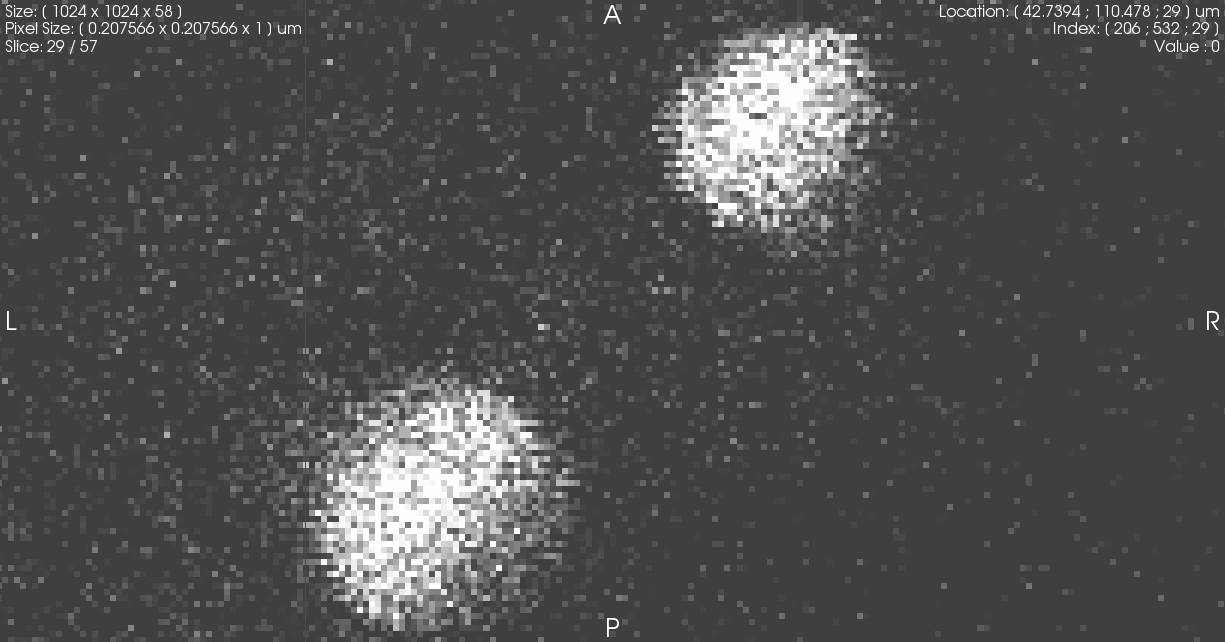
\includegraphics[width=0.7\textwidth]{pictures/InterlacingNuclei}}\\
  \subfloat[membrane channel]{\label{fig:InterlaceMembrane}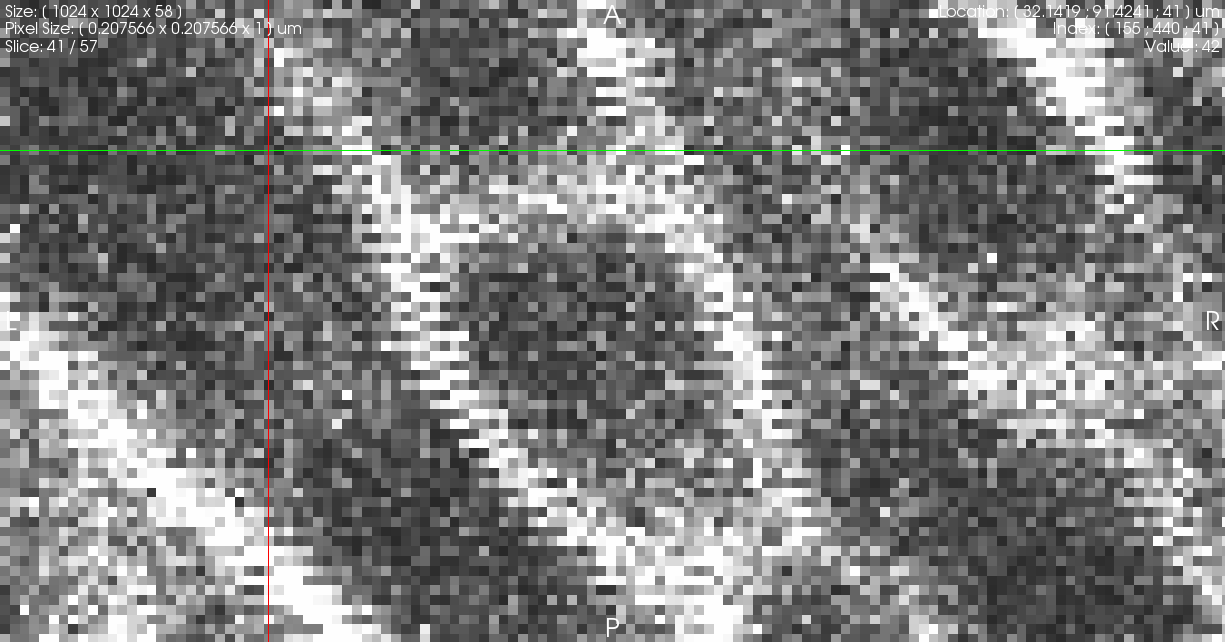
\includegraphics[width=0.7\textwidth]{pictures/InterlacingMembrane}}                
  \caption{Interlacing artifact on 2 photon confocal images. Views are x-y cuts of a 3D volume}
  \label{fig:InterlacingArtefact}
\end{figure}



\subsubsection{Anisotropy of images}


The datasets acquired in the Megason lab are anisotropic. As in the medical imaging domain, specialists are used to analyse images "slice by slice"
instead of considering them as a volume. They are worried about having a very detailed image in the x-y plan, and don't really worry about the other dimension.
This way of seeing things is wrong for images processing. A completely anisotropic image is very hard to process.
Non existing structures appear in the third dimension as illustrated figure~\ref{fig:Anysotropy}.
If a human brain with its understanding of the data may be able to interpret these structures, they lead most common algorithms to failure.

We can notice that nuclei seem to be stucked together and membrane's closure is almost always missing. This gives challenging a priori introduction problems.
\TODO{insert anisotropy examples}


\subsubsection{Noise}

There is much noise present in the datasets. Both membrane channel and nuclei channel are populated with non Gaussian noise.
The noise comes both from the microscope and electronics acquisition equipments, and from the biological sample that can be fluorescent in random locations.
The acquisition noise along z axis is decorrelated.
\TODO{get histograms of noise}

It could be interesting to study the response of the system to one small luminous point. The problem comes from the fact that depending on the phosphor used, the noise's statistics will differ.
\TODO{show noise in membrane and in nuclei}

\subsubsection{Low resolution of images}

The imaging process, combined with a too low resolution, leads to merged or missing structures. The nuclei channel displays very often clusters of merged nuclei when the membrane channel has information holes.
\TODO{show merged nuclei and holes in membrane}

\subsubsection{Point spread function}

The impulse response of the microscope is a noisy point spread function. That adds a deconvolution problem that can be treated together with the denoising problem. For simplicity reasons, searchers image with a very low resolution along the z axis, as the impulse function is spread out a lot along this axis.
\TODO{point spread function illustration}

\subsubsection{Complex structures}

The images we get are complex assembly of cells.
Some area being full of membrane, and others full with inter cellular liquid.
This is not a simple microscope slide with some well known cells, but a whole developing organism.


\TODO{show some fucked up functions}









\subsection{The megason lab imaging pipeline}

Dr Kishore Mosaliganti has been working for two years in the Megason lab, in order to develop new segmentation methods for fluorescent images.
He has been working on experiencing and developing diverse algorithms for nuclei and membrane detection and segmentation.
As presented is the previous section, the datasets in the Megason Lab are extremely challenging:
they are huge and present important drawbacks (resolution, noise) as they are provided for visual processing and not computer assisted processing.

As these datasets are very big, and four dimensional, it is not possible to use Matlab for easy prototyping and experiencing : 
most of the time, the very low resolution third dimension will considerably modify the results.
There is also a time issue : the datasets must be treated in an acceptable amount of time,
and that prevents us from using Matlab language that does not provide every optimized function that we need for 3D images visualization and processing.

This forces us to program and prototype in {\C++}. The standard library used for image processing in the Megason Lab is ITK. Kishore's algorithm are all coded with this library.
The data processing in ITK is represented by pipelines : a series of connected filters that perform image processing tasks.


Kishore studied several pipelines for nuclei and membrane segmentation.
For nuclei segmentation, an approach based on detection of nuclei, and region growing with the level set theory was used last year.
This year, a new approach based on nuclei detection and watershed algorithms is being used.
The algorithm used are standard and contour based for the detection of nuclei.
This leads to many errors in detection, due to the poor image quality. Right now, these errors are compensated after the segmentation step.

For membrane segmentation, Kishore is proposing a very good denoising technique based on anisotropic diffusion and tensor voting.
The reconstruction of the membrane structure is effective, even in low quality images. A segmentation step has to de implemented in top of it.

\subsection{The problem I am addressing}

I mainly focused on membrane segmentation prior to arriving in the Megason lab. This is a challenging problem, as shown by the data analysis : the membrane data is incomplete, noisy, three dimensional and anisotropic.

Having no prior knowledge on Kishore's data denoising, I focused on level sets techniques to segment the membrane.
The level set theory provides a very flexible framework for segmentation problems.
This is a generalisation of the fast marching algorithm. They are easily extensible to any dimension.
The drawbacks are that they are computationally intensive, and require theory learning prior to application.

Similarly to region growing algorithms, level set algorithms can be initialized to provide prior information.
I focused on growing a levelset function from cells center. For that purpose, we need a good cell localization.
I have been studying levels sets in Creatis, for the purpose of cell segmentation and had some results in two dimensions.
I was the considering that nuclei were already correctly detected and segmented, but when i arrived in the Megason Lab, I realized that before trying to segment the membrane using the techniques I studied in Creatis, I would need a correct cell nuclei detection.
We decided with Kishore that there was improvements to be brought to the cell nuclei detection algorithms.
















\fergfzgrertge 






ttttt

In the beginning of the internship, a new technique for nuclei detection was released.
As the one used in the Megason lab was not performing well enough, Kishore was willing to try and evaluate this new technique.



%
%  SEEDING
%


\section{Cell nuclei detection}

Cell nuclei shapes varies from spherical to curved ellipsoidal. As introduced above, the microscopy images are challenging, they are very noisy and anisotropic.
The main encountered difficulty is clustered nuclei that result from the point spread function of the microscope and the low resolution in the third dimension.

The algorithms used in the Megason lab for nuclei and membrane segmentation are based on an initialisation inside the nuclei.
Right now, a composite algorithm is used for detecting these nuclei. This algorithm is based on a combination of contour based algorithms :
Hough transform, \TOTO{Be clear : WHAT IS ZE TECHNIQUE? reading code is not instructive}
Those method provide us with landscapes (accumulation map for Hough transform, gradient vector flow tracking sinks, and finaly the intensity of smoothed nucleis) that we sum to combine the information fromo several sources. A local maxima detection is then performed on this resulting landscape.
This method gives good enough results for starting a watershed algorithm. Segmented regions that obviously don't correspond to a cell nucleus are eliminated. The final result of the segmentation process is evaluated.
\TODO{cite Kishore papers ?}


This is clear that for nuclei detection based segmentation methods, the nuclei detection has to be improved.
For that purpose we first implemented a new algorithm based on the Laplacian of Gaussian method.
Then we created an evaluation framework, to compare the results given by this new algorithm, and Kishore's.
We finally proposed a new method taking advantage of the cell membrane information.



\subsection{Bibliography on cell nuclei detection}

There are several papers dealing with cell nuclei detection, but very few are based on confocal images.
Another difficulty when doing such bibliography is the plethora of journals and the fact that Harvard Medical School doesn't have subscription for many imaging journals.
This restrains the scope of the bibliography.
I found several articles providing evaluation for their cell detection algorithm :
\begin{itemize}
  \item Constantinos G. et al\cite{•}, in his article about automatic counting of cancer cell nuclei in tissue sections propose an evaluaiton method based on two observers.
  They count the number of cells in ten images and the average number of cell counting error of the algorithm in percent the average number of cell present in the images is given (150). No information is provided on evaluating the cell nuclei position, or on the type of error : over detection or under detection ? The data are histological sections (2D).
  \item Gang Li et al\cite{}, in his article about 3D cell nuclei segmentation based on gradient flow tracking, presents a method for detecting and segmenting cell nuclei in 3D confocal
  datasets. The evaluation is done after the segmentation step and includes an elimination of detected nuclei that are too small. 
  They present the number of over segmented and under segmented cell nuclei, on a set of four images.
  \item P.S. Umesh Adiga et al\cite{}, in his article about segmentation of 3D histo-pathological images, present a method for segmenting cells in histological images 
  (which somehow close to nuclei in fluorescent images).
  The idea is to segment cells, using a watershed algorithm initialized on a simple cell center detection based on enhanced data (using morphological mathematics) and thresholding.
  The watershed algorithm is then run on such data and provides over segmented results. Those over segmented results are improved using constrained region merging. 
  The evaluation is done on 15 images and provides the original number of cells, and the number of detected cells for this algorithm.
  Two other algorithms are run on the same data to provide a comparison.
  \item Norberto Malpica et al\cite{•}, in his article about segmentation of clustered nuclei provides an evaluation based on two set of data : a training set (to adjust parameters of the algorithm), and a test set
\end{itemize}


Automatic detection of neurons in large cortical slices


%A "Plan of the internship"
%1 Goal (segment cells & membrane)
%2 Data presentation
%3 Where are we ? (membrane seg~0 cell seg needs lots of improvements)
%priority seeding imposed
%
%B Cell nuclei detection
% Intro
%bad seeding as of now, new ago, need for evaluation
%
%2 Biblio
%biblio on seeding evaluation
%
%3 Implementation
%implemantation … hard very hard (go through other's code forgotten already...)
%
%4 proposing
%new ago proposition new approach (based on membrane information)
%
%5 testing
%result of evaluation
%
%6 difficulties and future
%implementation big datasets 3D …
%future : merge results ? first : bad results everywhere : no more info for merging seedings...
%other ago based on wavelets? (as an opening)
%
%C Membrane segmentation
%  intro
%challenging need good cell detection...(but none present yet)
%1 biblio
%2 implementation (only 2D)
%3 result (only 2D)
%long very long but implementation can be greatly improved
%4 future
%not based on cell detection (start growing on the membrane)



%
%
%
%
%
%\section{Segmentation de la membrane cellulaire par ensembles de niveaux}
%
%Le but initial du PFE etait la segmentation de la membrane cellulaire. il s'agit d'une fine membrane séparant les multiples cellules. Elle s'étend sur tout le spécimen à analyser. Il s'agit donc d'un volume important et complexe.
%
%\subsection{Étude du problème}
%
%J'ai tout d'abord cherché à comprendre le problème posé : sur quelles données allaient se baser la détection, existe-t'il des solutions pour segmenter ce genre de données.
%
%\subsubsection{Les données}
%Les images sont acquises a travers un système optique. L'excitation par un laser entraine la fluorescence de certaines parties de la cellule, marquées par une molécule émettant de la lumière dans un spectre dépendant du marqueur utilisé.
%
%Le système a donc une réponse impulsionelle bien visible dans les données. Un point correspond grossièrement a une gaussienne étalée dans les trois dimensions de l'espace, et plus particulièrement selon l'axe perpendiculaire au plan de focalisation.
%
%Il existe aussi un bruit dû au dispositif électronique d'acquisition. De plus, la fluorescence n'étant pas répartie de manière homogène, il existe des "trous" et de la saturation dans les données.
%\TODO{inserer des images illustrant les problemes}
%
%
%J'ai choisi de me focaliser sur trois difficultés afin de trouver des solutions :
%\begin{description}
%  \item [problème du bruit] : quel filtrage appliquer aux images, afin de les débruiter.
%  \item [problème de l'absence de données] : comment introduire des à priori de forme de la membrane
%  pour palier à l'absence d'information ?
%  \item [problème de la non homogénéité des intensités]  : comment segmenter un objet
%  qui n'occupe pas les mêmes intensités selon sa position dans l'espace.
%\end{description}
%
%
%\subsection{Débruitage des données}
%Le bruit présent sur les images n'est pas gaussien. Il n'est pas répartis de la même manière dans toute l'image non plus. Je me suis donc focalisé sur des techniques de débruitage telles que le filtre médian, et plus généralement des filtres morphologiques.
%
%Le filtre médian donne de bons résultats, pour un temps de calcul inférieur aux filtres morphologiques (reconstruction par dilatation/erosion)
%
%\subsection{Segmentation de la membrane}
%
%\subsubsection{Utilisation de la théorie des ensembles de niveaux}
%
%L'outil choisi pour segmenter la paroi cellulaire, est base sur les ensembles de niveaux (levels-sets). Cette théorie consiste en l'évolution d'un front. Cette évolution est représentée par une fonction implicite qui évolue itérativement. Le front (bords de la zone segmentée) est souvent représenté par le niveau zéro de cette fonction implicite.
%Les Level sets, au travers de leur critère d'évolution, permettent d'avoir une grande flexibilité quand aux mesures a considerer lors de l'evolution du front. Cette évolution est représentée par un critère d'énergie, le problème de segmentation par level set est donc un problème d'optimisation.
%
%\subsection{des idees}
%
%
%
%
%
%
%idee de la mediane
%idee morphologie
%idee localisation
%\subsection{resultats}
%idee mediane
%idee morphologie
%idee localisation
%\subsection{travail futur}
%rapidite
%
%
%
%\section{Detection et localisation des cellules}
%
%Nous basons nos méthodes de segmentation sur une initialisation au centre des cellules. Nous avons donc besoin de détecter un maximum de cellules afin de trouver un point a l'intérieur de ces dernières. Des methodes ont ete proposees, cependant, chacune est adaptee a un type d'image particulier.
%Cels algorithmes de détection sont aussi souvent appelles algorithmes de "seeding" car ils permettent d'obtenir des points a partir desquels une segmentation peut etre initialisee, afin de delimiter les bordures des noyaux, ou les membranes cellulaires.
%
%\subsection{demarche}
%
%Nous avons developpe une methode combinant l'information provenant des noyaux et de la membrane des cellules. Cette methode doit etre evaluee, donc comparee a d'autres methodes existantes. Ce processus d'evaluation nous permettra aussi de trouver les points forts et les points faibles des algorithmes. Nous pourrons ainsi eventuellement utiliser des techniques de fusion d'information pour combiner les resultats de differents algorithmes.
%La creation d'un "framework" d'evaluation passe donc par plusieurs etapes : l'implementation des algorithmes existants, afin de les tester sur des images synthetiques puis reelles, la creation de criteres d'evaluation appropories, et l'observation des resultats. Nous avons aussi initié un travail afin de proposer une nouvelle methode de detection de cellules basee sur la decomposition en ondelettes.
%
%
%\subsection {description des algorithmes evalues}
%
%
%
%\subsubsection{chaine de traitement de l'image}
%
%partie commune
%Nous nous focalisons sur une classe d'algorithmes traitant l'information issue de l'image des noyaux cellulaires, apres une detection des zones d'interet (binarisation de l'image). Ces algorithmes fonctionnent aussi souvent avec une extraction de maxima locaux en dernier traitement.
%Nous choisissons d'utiliser la même binarisation, et la meme methode d'extraction de maximas locaux pour les deux algorithmes afin de focaliser l'etude sur la technique de detection des centres des noyaux.
%
%\subsubsection{description des algorithmes}
%\paragraph{le Laplacien de la Gaussienne ameliore}
%Nous avons decide d'implementer l'algorithme presente dans \cite{al2009improved}. La methode utilisee est celle du Laplacien de la Gaussienne (LoG). Une methode eprouveee qui s'est montree tres robuste dans d'autres applications telles la detection de points de reperes pour le recallage photographique.
%
%
%
%\paragraph{Kishore}
%
%\TODO{Ask Kishore more infos}
%
%
%\subsection {evaluation}
%%\begin{tabular}{|c|c|c|c|c|}
%%\hline  & Matching & UnMatching & Missed & Accuracy \\ 
%%\hline A1 & 10 & 3 & 1 & 71% \\ 
%%\hline A2 & 9 & 2 & 3 & 64% \\ 
%%\hline 
%%\end{tabular} 
%
%
%
%\subsection {conclusion}
%
%
%\subsection {proposition}
%
%
%
%\subsection {planning}
%
%
%\subsection{resultats}
%
%\subsection{proposition}
%
%
%
%
